\documentclass{../vespers-booklet}
\usepackage{multicol}

\begin{document}

% TODO: Update the title for the specific feast
\chapter*{Second Vespers of the Epiphany of Our Lord}

\vspace{0.5mm}

\begin{center}
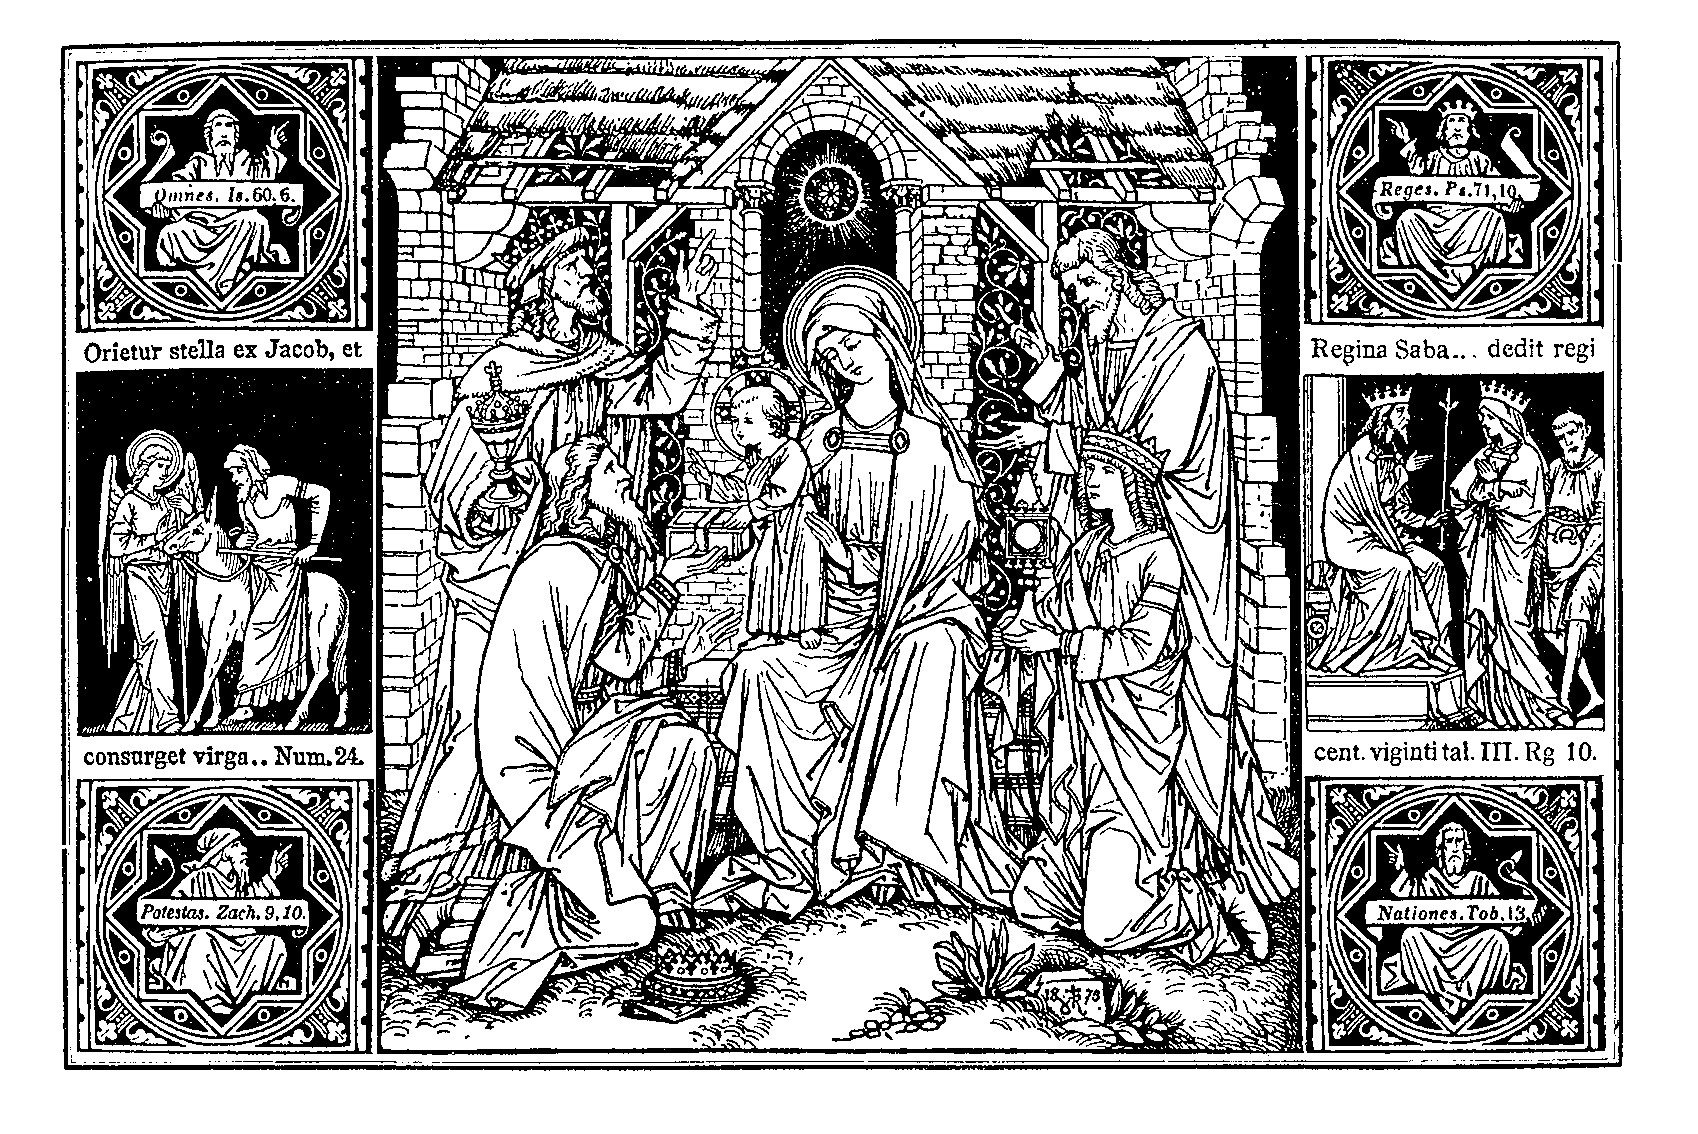
\includegraphics[width=\textwidth]{epiphany}
\end{center}

\vfill\pagebreak

%\section*{Beginning of the Office}

\begin{rubricbox}

{\color{red}When the Officiant kneels, all \textbf{kneel} and pray silently one \textit{Pater noster} (Our Father) and \textit{Ave Maria} (Hail Mary).
Then all make the sign of the cross with the Officiant as he intones:}

\end{rubricbox}

% TODO: Make sure that the tone of the deus adjutorium matches the season primarily and the solemnity of the feast secondarily
 \gresetinitiallines{1}
\gregorioscore{../common/deus-in-adjutorium-solemn}

\textit{
O God, come to my assistance.
{\color{red}\Vbar.}~O Lord, make haste to help me.
Glory be to the Father, and to the Son, and to the Holy Spirit,
as it was in the beginning, is now, and ever shall be, world without end. Amen.
Praise to Thee, O Lord, King of endless glory.}

\vfill\pagebreak

\section*{Psalm 109}

\textit{\textnormal{Ant. 1.} The Lord our Saviour, * begotten before the day-star, and before the ages, is this day made manifest in the world.
 \textnormal{Ps.} The Lord said to my Lord: * Sit thou at my right hand:}
 
 \begin{rubricbox}

{\color{red}All remain standing throughout the first antiphon.
After the psalm is intoned by the Cantor, all \textbf{sit} at the asterisk.}

\end{rubricbox}

\gresetinitiallines{1}
\gregorioscore{ps109-antiphon}

\gresetinitiallines{0}
\gregorioscore{ps109-intonation}

 \begin{latinenglishsection}

\latinenglish{

	2. Donec ponam inimícos \textbf{tu}os,~* scabéllum pedum \textit{tu}\textbf{ó}rum.

3. Virgam virtútis tuæ emíttet Dóminus ex \textbf{Si}on:~* domináre in médio inimicórum \textit{tu}\textbf{ó}rum.

4. Tecum princípium in die virtútis tuæ in splendóribus sanc\textbf{tó}rum:~* ex útero ante lucíferum gé\textit{nu}\textbf{i} te.

5. Jurávit Dóminus, et non p{\oe}nitébit \textbf{e}um:~* Tu es sacérdos in ætérnum secúndum órdinem \textit{Mel}\textbf{chí}sedech.

6. Dóminus a dextris \textbf{tu}is,~* confrégit in die iræ su\textit{æ} \textbf{re}ges.

7. Judicábit in natiónibus, implébit ru\textbf{í}nas:~*\\ conquassábit cápita in terra \textit{mul}\textbf{tó}rum.

8. De torrénte in via \textbf{bi}bet:~* proptérea exaltá\textit{bit} \textbf{ca}put.

9. {\color{red}\textit{(bow)}} Glória Patri, et \textbf{Fí}lio,~* et Spirítu\textit{i} \textbf{Sanc}to.

10. {\color{red}\textit{(rise)}} Sicut erat in princípio, et nunc, et \textbf{sem}per,~* et in s\'{\ae}cula sæculó\textit{rum}. \textbf{A}men.
 %%

}{
	% 1. The Lord said to my Lord: Sit thou at my right hand:

2. Until I make thy enemies thy footstool.
 
3. The Lord will send forth the sceptre of thy power out of Sion: rule thou in the midst of thy enemies.
 
4. With thee is the principality in the day of thy strength: in the brightness of the saints:
 from the womb before the day star I begot thee.
 
5. The Lord hath sworn, and he will not repent: Thou art a priest for ever according to the order of Melchisedech.
 
6. The Lord at thy right hand hath broken kings in the day of his wrath.

7. He shall judge among nations, he shall fill ruins: he shall crush the heads in the land of the many.

8. He shall drink of the torrent in the way: therefore shall he lift up the head. 

Glory be. %%
}

\end{latinenglishsection}

\gresetinitiallines{1}
\gregorioscore{ps109-antiphon}

%%

\section*{Psalm 110}

\textit{\textnormal{Ant. 2.} O Jerusalem, * thy light is come, and the glory of the Lord is risen upon thee, and the Gentiles shall walk in thy light. Alleluia.
 \textnormal{Ps.} I will praise thee, O Lord, with my whole heart; * in the council of the just, and in the congregation.}
 
 \begin{rubricbox}

{\color{red}All remain standing throughout the first antiphon.
After the psalm is intoned by the Cantor, all \textbf{sit} at the asterisk.}

\end{rubricbox}

\gresetinitiallines{1}
\gregorioscore{ps110-antiphon}

\vfill\pagebreak

\gresetinitiallines{0}
\gregorioscore{ps110-intonation}

 \begin{latinenglishsection}

\latinenglish{

	2. Magna \textit{ó}\textit{pe}\textit{ra} \textbf{Dó}\textbf{mi}ni:~* 
	exquisíta in omnes volun\textit{tá}\textit{tes} \textbf{e}jus.

3. Conféssio et magnificénti\textit{a} \textit{o}\textit{pus} \textbf{e}jus:~* 
	et justítia ejus manet in sǽ\textit{cu}\textit{lum} \textbf{sǽ}culi.

4. Memóriam fecit mirabílium suórum,~{\color{red}\GreDagger}\ miséricors et mi\textit{se}\textit{rá}\textit{tor} \textbf{Dó}\textbf{mi}nus:~* 
	escam dedit ti\textit{mén}\textit{ti}\textbf{bus} se.

5. Memor erit in sǽculum tes\textit{ta}\textit{mén}\textit{ti} \textbf{su}i:~* 
	virtútem óperum suórum annuntiábit pó\textit{pu}\textit{lo} \textbf{su}o:

6. Ut det illis here\textit{di}\textit{tá}\textit{tem} \textbf{gén}\textbf{ti}um:~* 
	ópera mánuum ejus véritas, \textit{et} \textit{ju}\textbf{dí}cium.

7. Fidélia ómnia mandáta ejus:~{\color{red}\GreDagger}\ confirmáta in \textit{sǽ}\textit{cu}\textit{lum} \textbf{sǽ}\textbf{cu}li,~* 
	facta in veritáte et \textit{æ}\textit{qui}\textbf{tá}te.

8. Redemptiónem misit \textit{pó}\textit{pu}\textit{lo} \textbf{su}o:~* 
	mandávit in ætérnum testa\textit{mén}\textit{tum} \textbf{su}um.

9. Sanctum, et terríbi\textit{le} \textit{no}\textit{men} \textbf{e}jus:~* 
	inítium sapiéntiæ \textit{ti}\textit{mor} \textbf{Dó}mini.

10. Intelléctus bonus ómnibus faci\textit{én}\textit{ti}\textit{bus} \textbf{e}um:~* 
	{\color{red}\textit{(stand)}} laudátio ejus manet in sǽ\textit{cu}\textit{lum} \textbf{sǽ}culi.

{\color{red}\textit{(bow)}} Glória \textbf{Pa}tri, et \textbf{Fí}lio,~*
	et Spirí\textit{tu}\textit{i} \textbf{Sanc}to.

{\color{red}\textit{(rise)}} Sicut erat in princípio, et \textbf{nunc}, et \textbf{sem}per,~*
	et in s\'{\ae}cula sæcu\textit{ló}\textit{rum}. \textbf{A}men. %%

}{
	 1. I will praise thee, O Lord, with my whole heart; in the council of the just: and in the congregation.
 
 2. Great are the works of the Lord: sought out according to all his wills.
 
 3. His work is praise and magnificence: and his justice continueth for ever and ever.
 
 4.  He hath made a remembrance of his wonderful works, being a merciful and gracious Lord: he hath given food to them that fear him. 	
 
 5. He will be mindful for ever of his covenant: he will shew forth to his people the power of his works.
 
 6. That he may give them the inheritance of the Gentiles: the works of his hands are truth and judgment.
 
 7. All his commandments are faithful: confirmed for ever and ever, made in truth and equity.
 
 8. He hath sent redemption to his people: he hath commanded his covenant for ever.
 
 9. Holy and terrible is his name: the fear of the Lord is the beginning of wisdom.
 
 10. A good understanding to all that do it: his praise continueth for ever and ever.  %%
}

\end{latinenglishsection}

\gresetinitiallines{1}
\gregorioscore{ps110-antiphon}

%%

\section*{Psalm 111}

\textit{\textnormal{Ant. 3.} When the wise men * had opened their treasures, they presented unto the Lord gold, frankincense, and myrrh. Alleluia.
 \textnormal{Ps.} Blessed is the man that feareth the Lord: * he shall delight exceedingly in his commandments.}
 
 \begin{rubricbox}

{\color{red}All remain standing throughout the first antiphon.
After the psalm is intoned by the Cantor, all \textbf{sit} at the asterisk.}

\end{rubricbox}

\gresetinitiallines{1}
\gregorioscore{ps111-antiphon}

\vfill\pagebreak

\gresetinitiallines{0}
\gregorioscore{ps111-intonation}

 \begin{latinenglishsection}

\latinenglish{

	2. Potens in terra erit \textbf{se}men \textbf{e}jus:~* generátio rectórum be\textit{ne}\textit{di}\textbf{cé}tur.

3. Glória, et divítiæ in \textbf{do}mo \textbf{e}jus:~* et justítia ejus manet in s\'{\ae}\textit{cu}\textit{lum} \textbf{s\'{\ae}}culi.

4. Exórtum est in ténebris \textbf{lu}men \textbf{rec}tis:~* miséricors, et miserá\textit{tor}, \textit{et} \textbf{jus}tus.

5. Jucúndus homo qui miserétur et cómmodat,~{\color{red}\GreDagger}\ dispónet sermónes suos \textbf{in} ju\textbf{dí}cio:~* quia in ætérnum non \textit{com}\textit{mo}\textbf{vé}bitur.

6. In memória ætérna \textbf{e}rit \textbf{jus}tus:~* ab auditióne mala \textit{non} \textit{ti}\textbf{mé}bit.

7. Parátum cor ejus speráre in Dómino,~{\color{red}\GreDagger}\ confirmátum \textbf{est} cor \textbf{e}jus:~* non commovébitur donec despíciat ini\textit{mí}\textit{cos} \textbf{su}os.

8. Dispérsit, dedit paupéribus:~{\color{red}\GreDagger}\ justítia ejus manet in \textbf{s\'{\ae}}culum \textbf{s\'{\ae}}culi,~* cornu ejus exaltábi\textit{tur} \textit{in} \textbf{gló}ria.

9. Peccátor vidébit, et irascétur,~{\color{red}\GreDagger}\ déntibus suis fremet \textbf{et} ta\textbf{bé}scet:~* desidérium peccató\textit{rum}\\ \textit{per}\textbf{í}bit.

\textit{(bow)} Glória \textbf{Pa}tri, et \textbf{Fí}lio,~* et Spirí\textit{tu}\textit{i} \textbf{Sanc}to.

\textit{(rise)} Sicut erat in princípio, et \textbf{nunc}, et \textbf{sem}per,~* et in s\'{\ae}cula sæcu\textit{ló}\textit{rum}. \textbf{A}men. %%

}{
	1. Blessed is the man that feareth the Lord: he shall delight exceedingly in his commandments.

2. His seed shall be mighty upon earth: the generation of the righteous shall be blessed.

3. Glory and wealth shall be in his house: and his justice remaineth for ever and ever.

4. To the righteous a light is risen up in darkness: he is merciful, and compassionate and just.

5. Acceptable is the man that sheweth mercy and lendeth: he shall order his words with judgment:
because he shall not be moved for ever.

6. The just shall be in everlasting remembrance: he shall not fear the evil hearing.

7. His heart is ready to hope in the Lord: his heart is strengthened, he shall not be moved until he look over his enemies.

8. He hath distributed, he hath given to the poor: his justice remaineth for ever and ever: his horn shall be exalted in glory.

9. The wicked shall see, and shall be angry, he shall gnash with his teeth and pine away: the desire of the wicked shall perish.  %%
}

\end{latinenglishsection}

\gresetinitiallines{1}
\gregorioscore{ps111-antiphon}

%%

\section*{Psalm 112}

\textit{\textnormal{Ant. 4.} O ye seas and floods, * bless ye the Lord. O ye wells, bless ye the Lord. Alleluia.
 \textnormal{Ps.} Praise the Lord, ye children: * praise ye the name of the Lord.}
 
 \begin{rubricbox}

{\color{red}All remain standing throughout the first antiphon.
After the psalm is intoned by the Cantor, all \textbf{sit} at the asterisk.}

\end{rubricbox}

\gresetinitiallines{1}
\gregorioscore{ps112-antiphon}

\gresetinitiallines{0}
\gregorioscore{ps112-intonation}

 \begin{latinenglishsection}

\latinenglish{

	2. \textit{(bow)} Sit nomen Dómini \textit{be}\textit{ne}\-\textbf{díc}tum,~* ex hoc nunc, et \textit{us}\textit{que} \textit{in} \textbf{s\'{\ae}}\textbf{cu}lum.

3. A solis ortu usque \textit{ad} \textit{oc}\textbf{cá}sum,~* laudábi\textit{le} \textit{no}\textit{men} \textbf{Dó}\textbf{mi}ni.

4. Excélsus super omnes \textit{gen}\textit{tes} \textbf{Dó}minus,~* et super cælos \textit{gló}\textit{ri}\textit{a} \textbf{e}jus.

5. Quis sicut Dóminus, Deus noster, qui in \textit{al}\textit{tis} \textbf{há}bitat,~* et humília réspicit in cæ\textit{lo} \textit{et} \textit{in} \textbf{ter}ra?

6. Súscitans a \textit{ter}\textit{ra} \textbf{ín}opem,~* et de stércore \textit{é}\textit{ri}\textit{gens} \textbf{páu}\textbf{pe}rem:

7. Ut cóllocet eum \textit{cum} \textit{prin}\textbf{cí}pibus,~* cum princípibus \textit{pó}\textit{pu}\textit{li} \textbf{su}i.

8. Qui habitáre facit stéri\textit{lem} \textit{in} \textbf{do}mo,~* matrem fili\textit{ó}\textit{rum} \textit{læ}\textbf{tán}tem.

\textit{(bow)} Glória Pa\textit{tri}, \textit{et} \textbf{Fí}lio,~* et Spi\textit{rí}\textit{tu}\textit{i} \textbf{Sanc}to.

\textit{(rise)} Sicut erat in princípio, et \textit{nunc}, \textit{et} \textbf{sem}per,~* et in s\'{\ae}cula sæ\textit{cu}\textit{ló}\textit{rum}. \textbf{A}men. %%

}{
	%1. Praise the Lord, ye children: praise ye the name of the Lord.
 	
2. Blessed be the name of the Lord, from henceforth now and for ever.
 	
3. From the rising of the sun unto the going down of the same, the name of the Lord is worthy of praise.
 	
4. The Lord is high above all nations; and his glory above the heavens.
 	
5.Who is as the Lord our God, who dwelleth on high, and looketh down on the low things in heaven and in earth?
 	
6. Raising up the needy from the earth, and lifting up the poor out of the dunghill:
 	
7. That he may place him with princes, with the princes of his people.
 	
8. Who maketh a barren woman to dwell in a house, the joyful mother of children. 

Glory be. %%
}

\end{latinenglishsection}

\gresetinitiallines{1}
\gregorioscore{ps112-antiphon}

\vfill\pagebreak

%%

\section*{Psalm 113}

\textit{\textnormal{Ant. 5.} This star shineth * as a flame of fire, and pointeth out God, the King of kings: the Wise Men beheld it, and offered gifts unto the great King.
 \textnormal{Ps.} When Israel went out of Egypt, * the house of Jacob from a barbarous people:}
 
 \begin{rubricbox}

{\color{red}All remain standing throughout the first antiphon.
After the psalm is intoned by the Cantor, all \textbf{sit} at the asterisk.}

\end{rubricbox}

\gresetinitiallines{1}
\gregorioscore{ps113-antiphon}

\gresetinitiallines{0}
\gregorioscore{ps113-intonation}

 \begin{latinenglishsection}

\latinenglish{

	2. Facta est Jud\'{\ae}a sanctifi\textbf{cá}tio \textbf{eG}jus,~* 
	Israël pot\textbf{és}tas \textbf{e}jus.

3. Mare \textbf{vi}dit, et \textbf{fu}git:~* 
	Jordánis convérsus \textbf{est} re\textbf{trór}sum.

4. Montes exsultavérunt \textbf{ut} a\textbf{rí}\textbf{e}tes,~* 
	et colles sicut \textbf{a}gni \textbf{ó}vium.

5. Quid est tibi, mare, \textbf{quod} fu\textbf{gís}ti:~* 
	et tu, Jordánis, quia convérsus \textbf{es} re\textbf{trór}sum?

6. Montes, exsultástis \textbf{sic}ut a\textbf{rí}\textbf{e}tes,~* 
	et colles, sicut \textbf{a}gni \textbf{ó}vium.

7. A fácie Dómini \textbf{mo}ta est \textbf{ter}ra,~* 
	a fácie \textbf{De}i \textbf{Ja}cob.

8. Qui convértit petram in \textbf{sta}gna a\textbf{quá}rum,~* 
	et rupem in \textbf{fon}tes a\textbf{quá}rum.

9. Non nobis, Dómi\textbf{ne}, non \textbf{no}bis:~* 
	sed nómini \textbf{tu}o da \textbf{gló}riam.

10. Super misericórdia tua, et veri\textbf{tá}te \textbf{tu}a:~* 
	nequándo dicant gentes: Ubi est \textbf{De}us e\textbf{ó}rum?

11. Deus autem \textbf{nos}ter in \textbf{cæ}lo:~* 
	ómnia quæcúmque \textbf{vó}luit, \textbf{fe}cit.

12. Simulácra géntium ar\textbf{gén}tum, et \textbf{au}rum,~* 
	ópera \textbf{má}nuum\\ \textbf{hó}minum.

13. Os habent, et \textbf{non} lo\textbf{quén}tur:~* 
	óculos habent, et \textbf{non} vi\textbf{dé}bunt.

14. Aures habent, \textbf{et} non \textbf{áu}\textbf{di}ent:~* 
	nares habent, et non \textbf{o}do\textbf{rá}bunt.

15. Manus habent, et non palpábunt:~{\color{red}\GreDagger}\ pedes habent, et non \textbf{am}bu\textbf{lá}bunt:\\ * 
	non clamábunt in \textbf{gút}ture \textbf{su}o.

16. Símiles illis fiant qui \textbf{fá}ciunt \textbf{e}a:~* 
	et omnes qui con\textbf{fí}dunt in \textbf{e}is.

17. Domus Israël spe\textbf{rá}vit in \textbf{Dó}\textbf{mi}no:~* 
	adjútor eórum et\\ pro\textbf{téc}tor e\textbf{ó}rum est,

18. Domus Aaron spe\textbf{rá}vit in\\ \textbf{Dó}\textbf{mi}no:~* 
	adjútor eórum et\\ pro\textbf{téc}tor e\textbf{ó}rum est,

19. Qui timent Dóminum,\\ spera\textbf{vé}runt in \textbf{Dó}\textbf{mi}no:~* 
	adjútor eórum et pro\textbf{téc}tor e\textbf{ó}rum est.

20. Dóminus memor \textbf{fu}it \textbf{nos}tri:~* 
	et bene\textbf{dí}xit \textbf{no}bis:

21. Benedíxit \textbf{dó}mui \textbf{Is}\textbf{ra}ël:~* 
	benedíxit \textbf{dó}mui \textbf{A}aron.

22. Benedíxit ómnibus, qui \textbf{ti}ment \textbf{Dó}\textbf{mi}num,~* 
	pusíllis \textbf{cum} ma\textbf{jó}ribus.

23. Adjíciat \textbf{Dó}minus \textbf{su}\textbf{per} vos:~* 
	super vos, et super \textbf{fí}lios \textbf{ves}tros.

24. Benedícti \textbf{vos} a \textbf{Dó}\textbf{mi}no,~* 
	qui fecit \textbf{cæ}lum, et \textbf{ter}ram.

25. Cælum \textbf{cæ}li \textbf{Dó}\textbf{mi}no:~* 
	terram autem dedit \textbf{fí}liis \textbf{hó}minum.

26. Non mórtui lau\textbf{dá}bunt te, \textbf{Dó}\textbf{mi}ne:~* 
	neque omnes, qui\\ descéndunt \textbf{in} in\textbf{fér}num.

27. Sed nos qui vívimus,\\ bene\textbf{dí}cimus \textbf{Dó}\textbf{mi}no,~* 
	{\color{red}\textit{(stand)}} ex hoc nunc et \textbf{us}que in \textbf{s\'{\ae}}culum.

28. {\color{red}\textit{(bow)}} Glória \textbf{Pa}tri, et \textbf{Fí}\textbf{li}o,~* 
	et Spi\textbf{rí}tui \textbf{Sanc}to.

29. {\color{red}\textit{(rise)}} Sicut erat in princípio, et \textbf{nunc}, et \textbf{sem}per,~* 
	et in s\'{\ae}cula sæcu\textbf{ló}rum. \textbf{A}men.
 %%

}{
	1. When Israel went out of Egypt, the house of Jacob from a barbarous people:

2. Judea was made his sanctuary, Israel his dominion.

3. The sea saw and fled: Jordan was turned back.

4. The mountains skipped like rams, and the hills like the lambs of the flock.

5. What ailed thee, O thou sea, that thou didst flee: and thou, O Jordan, that thou wast turned back?

6. Ye mountains, that ye skipped like rams, and ye hills, like lambs of the flock?

7. At the presence of the Lord the earth was moved, at the presence of the God of Jacob:

8. Who turned the rock into pools of water, and the stony hill into fountains of waters.

9. Not to us, O Lord, not to us; but to thy name give glory.

10. For thy mercy, and for thy truth's sake: lest the gentiles should say: Where is their God?

11. But our God is in heaven: he hath done all things whatsoever he would.

12. The idols of the gentiles are silver and gold, the works of the hands of men.

13. They have mouths and speak not: they have eyes and see not.

14. They have ears and hear not: they have noses and smell not.

15. They have hands and feel not: they have feet and walk not: neither shall they cry out through their throat.

16. Let them that make them become like unto them: and all such as trust in them.

17. The house of Israel hath hoped in the Lord: he is their helper and their protector.

18. The house of Aaron hath hoped in the Lord: he is their helper and their protector.

19. They that fear the Lord hath hoped in the Lord: he is their helper and their protector.

20. The Lord hath been mindful of us, and hath blessed us.

21. He hath blessed the house of Israel: he hath blessed the house of Aaron.

22. He hath blessed all that fear the Lord, both little and great.

23. May the Lord add blessings upon you: upon you, and upon your children.

24. Blessed be you of the Lord, who made heaven and earth.

25. The heaven of heaven is the Lord's: but the earth he has given to the children of men.

26. The dead shall not praise thee, O Lord: nor any of them that go down to hell.

27. But we that live bless the Lord: from this time now and for ever. %%
}

\end{latinenglishsection}

%\vfill\pagebreak

\gresetinitiallines{1}
\gregorioscore{ps113-antiphon}

\vfill\pagebreak

\section*{Little Chapter (Isaiah 60:1)}

\textit{\color{red}The Officiant leads the Little Chapter:}

\begin{latinenglishsection}

\latinenglish{
	Surge, illumináre Jerúsalem, {\color{red}\GreDagger} quia venit \textit{lumen} \textbf{tu}um, et glória Dómini super te orta est.
	{\color{red}\Rbar.}~Deo grátias.
}{
	Arise, be enlightened, O Jerusalem: for thy light is come, and the glory of the Lord is risen upon thee.
	{\color{red}\Rbar.}~Thanks be to God.
}

\end{latinenglishsection}

\section*{Hymn}

\textit{\color{red}The Cantor leads the hymn:}

\gresetinitiallines{1}
\gregorioscore{../hymns/crudelis-herodes-deum}

{\itshape
1. Why, impious Herod, vainly fear
That Christ the Saviour cometh here?
He takes no earthly realms away
Who gives the crown that lasts for aye.

2. To greet His birth the Wise Men went,
Led by the star before them sent;
Called on by light, towards light they pressed,
And by their gifts their God confessed.

3. In holy Jordan's purest wave
The heavenly Lamb vouchsafed to lave;
That He, to whom was sin unknown,
Might cleanse His people from their own.

4. New miracle of power divine!
The water reddens into wine:
He spake the word: and poured the wave
In other streams than nature gave.

5. All glory, Lord, to thee we pay
For thine Epiphany to-day:
All glory, as is ever meet,
To Father and to Paraclete.
Amen.
}

\textit{\color{red}The Cantor says the following before all reply afterwards:}

\gresetinitiallines{0}
\gabcsnippet{
(c3) <c><sp>V/</sp>.</c> Re(h)ges(h) Thar(h)sis(h) et(h) ín(h)su(h)læ(h) mú(h)ne(h)ra(h) óf(h)fe(h)rent.(g'_/hvGF'E/fgf.) (::)
}

\gresetinitiallines{0}
\gabcsnippet{
(c3) <c><sp>R/</sp>.</c> Re(h)ges(h) A(h)ra(h)bum(h) et(h) Sa(h)ba(h) do(h)na(h) ad(h)dúc(h)ent.(g'_/hvGF'E/fgf.) (::)
}

\textit{{\color{red}\Vbar.}~The kings of Tarshish and of the isles shall bring presents.
{\color{red}\Rbar.}~The kings of Arabia and Saba shall offer gifts..}

%TODO: Verify that the magnificat antiphon is correct and match the mangificat intonation and pointed text with the tone

\section*{Magnificat}

\textit{\textnormal{Ant Magn.} Behold a faithful and prudent servant, whom the Lord has set over His household.
\textnormal{Cant.} My soul doth magnify the Lord: and my spirit hath rejoiced in God my Saviour.}

\begin{rubricbox}

{\color{red}The Cantor leads by intoning the antiphon and the first verse.}

\end{rubricbox}

\gresetinitiallines{1}
\gregorioscore{magnificat-antiphon-only}

\begin{rubricbox}

{\color{red}All \textbf{stand} and make the sign of the cross with the Cantor.}

\end{rubricbox}

\vfill\pagebreak

\gresetinitiallines{0}
\gregorioscore{magnificat-intonation}

 \begin{latinenglishsection}

\latinenglish{	
3. Quia respéxit humilitátem \textit{an}\textit{cíl}\textit{læ} \textbf{su}æ:~* 
	ecce enim ex hoc beátam me dicent omnes gene\textit{ra}\textit{ti}\textbf{ó}nes.

4. Quia fecit mihi \textit{ma}\textit{gna} \textit{qui} \textbf{pot}\textbf{ens} est:~* 
	et sanctum \textit{no}\textit{men} \textbf{e}jus.

5. Et misericórdia ejus a progéni\textit{e} \textit{in} \textit{pro}\textbf{gé}\textbf{ni}es~* 
	timén\textit{ti}\textit{bus} \textbf{e}um.

6. Fecit poténtiam in \textit{brá}\textit{chi}\textit{o} \textbf{su}o:~* 
	dispérsit supérbos mente \textit{cor}\textit{dis} \textbf{su}i.

7. Depósuit pot\textit{én}\textit{tes} \textit{de} \textbf{se}de,~* 
	et exal\textit{tá}\textit{vit} \textbf{hú}miles.

8. Esuriéntes \textit{im}\textit{plé}\textit{vit} \textbf{bo}nis:~* 
	et dívites dimí\textit{sit} \textit{in}\textbf{á}nes.

9. Suscépit Israël \textit{pú}\textit{e}\textit{rum} \textbf{su}um,~* 
	recordátus misericór\textit{di}\textit{æ} \textbf{su}æ.

10. Sicut locútus est \textit{ad} \textit{pa}\textit{tres} \textbf{nos}tros,~* 
	Abraham et sémini e\textit{jus} \textit{in} \textbf{s\'{\ae}}cula.
}{	
	1. My soul doth magnify the Lord.

2. And my spirit hath rejoiced in God my Saviour.

3. Because he hath regarded the humility of his handmaid; for behold from henceforth all generations shall call me blessed.

4. Because he that is mighty, hath done great things to me; and holy is his name.

5. And his mercy is from generation unto generations, to them that fear him.

6. He hath shewed might in his arm: he hath scattered the proud in the conceit of their heart.

7. He hath put down the mighty from their seat, and hath exalted the humble.

8. He hath filled the hungry with good things; and the rich he hath sent empty away.

9. He hath received Israel his servant, being mindful of his mercy: 

10. As he spoke to our fathers, to Abraham and to his seed for ever. 
}

\end{latinenglishsection}

\textit{\color{red}(bow)} Glória \textit{Pa}\textit{tri}, \textit{et} \textbf{Fí}\textbf{li}o,~* 
	et Spirí\textit{tu}\textit{i} \textbf{Sanc}to.

\textit{\color{red}(rise)} Sicut erat in princípio, \textit{et} \textit{nunc}, \textit{et} \textbf{sem}per,~* 
	et in s\'{\ae}cula sæcu\textit{ló}\textit{rum}. \textbf{A}men. 
	
\vfill\pagebreak

\gresetinitiallines{1}
\gregorioscore{magnificat-antiphon-only}

\vfill\pagebreak

\section*{Collect}

\textit{\color{red}The Officiant leads the collect:}

\begin{latinenglishsection}

\latinenglish{
	{\color{red}\Vbar.}~Dómine exáudi oratiónem meam.\\
	{\color{red}\Rbar.}~Et clamor meus ad te véniat.
	
	Orémus.
	Deus, qui hodiérna die Unigénitum tuum géntibus stella duce revelásti: concéde propítius; ut qui jam te ex fide cognóvimus, usque ad contemplándam spéciem tuæ celsitúdinis perducámur.
	Per eúmdem Dóminum nostrum Jesum Christum Fílium tuum, qui tecum vivit et regnat in unitáte Spíritus Sancti, Deus, per ómnia s\'{\ae}cula sæculórum.
	{\color{red}\Rbar.}~Amen.
}{
	{\color{red}\Vbar.} Lord, hear my prayer.
	{\color{red}\Rbar.}~And let my cry come unto Thee.
	
	Let us pray.
	O God, Who by the leading of a star didst, as on this day, manifest thine Only-begotten Son to the Gentiles, mercifully grant that we, which know thee now by faith, may after this life have the fruition of thy glorious Godhead:
	Through the same Jesus Christ, thy Son, Our Lord, Who liveth and reigneth with thee in the unity of the Holy Ghost, God, world without end.
	{\color{red}\Rbar.}~Amen.
}
\end{latinenglishsection}

%\textit{\color{red}For commemorations, the Cantor intones the antiphon and says the responsorial prayer afterwards. The Officiant prays the associated collect.}

\textit{\color{red}The Officiant leads the following:}

\begin{latinenglishsection}
\latinenglish{
	{\color{red}\Vbar.}~Dómine exáudi oratiónem meam.\\
	{\color{red}\Rbar.}~Et clamor meus ad te véniat.
}{
	{\color{red}\Vbar.}~Lord, hear my prayer. {\color{red}\Rbar.}~And let my cry come unto Thee.
	{\color{red}\Vbar.}~Let us bless the Lord. {\color{red}\Rbar.}~Thanks be to God.
}

\end{latinenglishsection}

\textit{\color{red}The Cantor leads the Benedicamus:}

\gresetinitiallines{1}
\gregorioscore{../common/benedicamus-2v-solem}

\textit{\color{red}The Officiant leads the following:}

\begin{latinenglishsection}

\latinenglish{
	{\color{red}\Vbar.} Fidélium ánimæ, per\\ misericórdiam Dei, requiéscant in pace. \\
	{\color{red}\Rbar.} Amen.
}{
	May the souls of the faithful departed, through the mercy of God, rest in peace. {\color{red}\Rbar.}~Amen.
}

\latinenglish{
	Pater noster \textit{(silently)}.
}{
	Our Father\dots
}

\latinenglish{
	{\color{red}\Vbar.} Dóminus det nobis suam pacem. \\
	{\color{red}\Rbar.} Et vitam ætérnam. Amen.
}{
	May the Lord grant us his peace. {\color{red}\Rbar.}~And life eternal. Amen.
}

\end{latinenglishsection}

%TODO: Add the Marian Anthem for the season and verify that the oration afterwards is correct

\section*{Marian Anthem}

\textit{\color{red}The Cantor leads the Marian anthem and responses afterwards; the Officiant leads the ending collect:}

\gresetinitiallines{1}
\gregorioscore{../marian-anthems/ave-regina-caelorum-solemn}

{\itshape
	Hail, O Queen of Heaven enthroned.
	Hail, by angels mistress owned.
	Root of Jesse, Gate of Morn
	whence the world's true light was born.
	
	Glorious Virgin, Joy to thee,
	loveliest whom in heaven they see;
	fairest thou, where all are fair,
	plead with Christ our souls to spare.
}

\begin{latinenglishsection}

\latinenglish{
	{\color{red}\Vbar.} Dignáre me laudáre te, Virgo sacráta.\\
	{\color{red}\Rbar.} Da mihi virtútem contra hostes tuos.
	
	Orémus.
	Concéde, miséricors Deus, fragilitáti nostræ præsídium:
	ut qui sanctæ Dei Genitrícis memóriam ágimus;
	intercessiónis ejus auxílio, a nostris iniquitátibus resurgámus.
	Per eúmdem Christum Dóminum nostrum.
	{\color{red}\Rbar.}~Amen.
}{
	{\color{red}\Vbar.}Vouchsafe that I may praise thee, O sacred Virgin.
	{\color{red}\Rbar.}~Give me stength against thine enemies.
	
	Let us pray.
	Grant, O merciful God, to our weak natures Thy protection,
	that we who commemorate the holy Mother of God may,
	by the help of her intercession, arise from our iniquities.
	Through the same Christ our Lord.
	{\color{red}\Rbar.}~Amen.
}
\end{latinenglishsection}

\textit{\color{red}The Officiant says the following in a low recto tono:}

\begin{latinenglishsection}

\latinenglish{
	{\color{red}\Vbar.} Divínum auxílium máneat semper nobíscum.\\
	{\color{red}\Rbar.} Amen.
}{
	{\color{red}\Vbar.}~May the divine assistance remain always with us.
	{\color{red}\Rbar.}~Amen.
}
\end{latinenglishsection}

\begin{rubricbox}

{\color{red} After the Office, all \textbf{kneel} and pray in silence for a time.}

\end{rubricbox}

\end{document}